\let\negmedspace\undefined
\let\negthickspace\undefined
\documentclass[journal]{IEEEtran}
\usepackage[a4paper, margin=10mm, onecolumn]{geometry}
%\usepackage{lmodern} % Ensure lmodern is loaded for pdflatex
\usepackage{tfrupee} % Include tfrupee package
\setlength{\headheight}{1cm} % Set the height of the header box
\setlength{\headsep}{0mm}   % Set the distance between the header box and the top of the text
\usepackage{gvv-book}
\usepackage{gvv}
\usepackage{cite}
\usepackage{amsmath,amssymb,amsfonts,amsthm}
\usepackage{algorithmic}
\usepackage{graphicx}
\usepackage{float}
\usepackage{textcomp}
\usepackage{xcolor}
\usepackage{txfonts}
\usepackage{listings}
\usepackage{enumitem}
\usepackage{mathtools}
\usepackage{gensymb}
\usepackage{comment}
\usepackage[breaklinks=true]{hyperref}
\usepackage{tkz-euclide} 
\usepackage{listings}
% \usepackage{gvv}                                       
\def\inputGnumericTable{}                                
\usepackage[latin1]{inputenc}                               
\usepackage{color}                                       
\usepackage{array}                                       
\usepackage{longtable}                                   
\usepackage{calc}                                        
\usepackage{multirow}                                    
\usepackage{hhline}                                      
\usepackage{ifthen}                                      
\usepackage{lscape}
\usepackage{tikz}
\usetikzlibrary{patterns}
\begin{document}
\bibliographystyle{IEEEtran}
\vspace{3cm}
\title{4.7.51}
\author{ee25btech11054-S.Harsha Vardhan Reddy}
\maketitle
% \maketitle
% \newpage
% \bigskip
{\let\newpage\relax\maketitle}
\renewcommand{\thefigure}{\theenumi}
\renewcommand{\thetable}{\theenumi}
\setlength{\intextsep}{10pt} % Space between text and floats
\numberwithin{equation}{enumi}
\numberwithin{figure}{enumi}
\renewcommand{\thetable}{\theenumi}
\begin{problem}[4.7.51]
Find the equation of the plane passing through the point ( -1, 3, 2) and perpendicular to each of the planes $x + 2y + 3z = 5$ and $3x + 3y + z = 0$.
\end{problem}

\solution
The normal vectors to the given planes are $\vec{n_1} = \myvec{1 \\ 2 \\ 3}$ and $\vec{n_2} = \myvec{3 \\ 3 \\ 1}$.

Let the normal vector of the required plane be $\vec{n} = \myvec{n_1 \\ n_2 \\ n_3}$. Since the required plane is perpendicular to both given planes, its normal vector $\vec{n}$ must be orthogonal to both $\vec{n_1}$ and $\vec{n_2}$. This gives the following homogeneous system of linear equations:
\begin{align}
\vec{n_1}^\top \vec{n} &= n_1 + 2n_2 + 3n_3 = 0 \label{eq:4.7.51.1} \\
\vec{n_2}^\top \vec{n} &= 3n_1 + 3n_2 + n_3 = 0 \label{eq:4.7.51.2}
\end{align}
To solve this system, we form the augmented matrix and reduce it. The final reduced row echelon form is:
\begin{equation}
\left(\begin{array}{ccc|c} 1 & 2 & 3 & 0 \\ 3 & 3 & 1 & 0 \end{array}\right) \quad \xrightarrow{\text{Row Reduce}} \quad \left(\begin{array}{ccc|c} 1 & 0 & -7/3 & 0 \\ 0 & 1 & 8/3 & 0 \end{array}\right)
\end{equation}
From the reduced form, we have:
\begin{align}
n_1 - \frac{7}{3}n_3 &= 0 \implies n_1 = \frac{7}{3}n_3 \nonumber \\
n_2 + \frac{8}{3}n_3 &= 0 \implies n_2 = -\frac{8}{3}n_3 \nonumber
\end{align}
The solution space for $\vec{n}$ is spanned by the vector $\myvec{7/3 \\ -8/3 \\ 1}$. We can choose any non-zero scalar multiple of this vector for our normal. Letting the free variable $n_3 = -3$ gives a simple integer vector:
\begin{equation}
\vec{n} = \myvec{-7 \\ 8 \\ -3}
\label{eq:4.7.51.3}
\end{equation}
The equation of the required plane passes through the point $\vec{P_0} = \myvec{-1 \\ 3 \\ 2}$ and has the normal vector $\vec{n}$. The equation is $\vec{n}^\top \vec{p} = \vec{n}^\top \vec{P_0}$.
\begin{equation}
c = \myvec{-7 & 8 & -3}^\top \myvec{-1 \\ 3 \\ 2} = 7 + 24 - 6 = 25
\label{eq:4.7.51.4}
\end{equation}
Thus, the equation of the plane is:
\begin{align}
\myvec{7 & -8 & 3}
\myvec{x \\ y \\ z}
= -25
\end{align}

\begin{figure}[h]
    \centering
    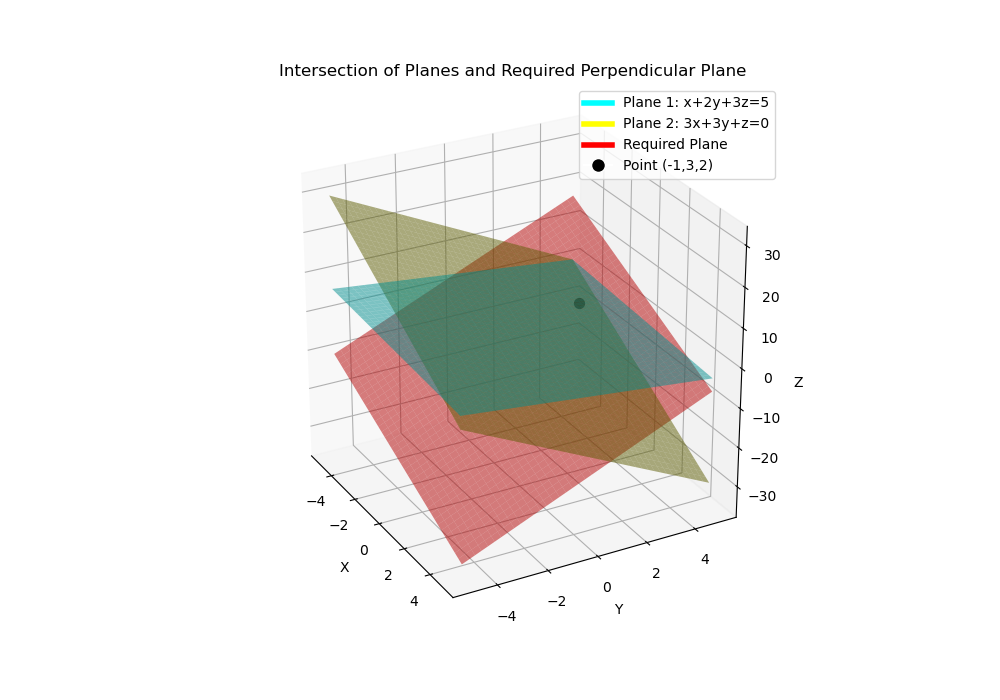
\includegraphics[width=1.1\linewidth]{figs/plot8.png}
    \caption{}
    \label{fig:placeholder}
\end{figure}
\end{document}